% $Header: /Users/joseph/Documents/LaTeX/beamer/solutions/conference-talks/conference-ornate-20min.en.tex,v 90e850259b8b 2007/01/28 20:48:30 tantau $

\documentclass{beamer}

%\usepackage{CJK}
%\usepackage{CJK,CJKnumb}
%\usepackage{ctex}
\usepackage[english]{babel}
\usepackage[utf8]{inputenc}
%\usepackage{setspace}
\usepackage{graphicx}
\usepackage{bm}
\usepackage{textpos}
\usepackage{algpseudocode}
\usepackage{algorithm}
\usepackage{url}
\usepackage{multirow}
\usepackage{threeparttable}
\usepackage{hyperref}
\usepackage{times}
\usepackage[T1]{fontenc}
\usepackage{ulem,tikz}
% Or whatever. Note that the encoding and the font should match. If T1
% does not look nice, try deleting the line with the fontenc.
\usepackage{stfloats}
\usepackage[caption=false,font=scriptsize]{subfig}
%\usepackage[font=scriptsize,labelfont=scriptsize]{caption}

%\setbeameroption{show notes on second screen}
%\setbeamertemplate{note page}[compress]
\usepackage{csquotes}
%\usepackage[style=numeric-comp,autocite=footnote,citetracker=true,maxnames=1,sorting=none,babel=hyphen,hyperref=true,backend=biber]{biblatex}
\usepackage[style=numeric-comp,autocite=footnote,citetracker=true,maxnames=1,sorting=none]{biblatex}
%\usepackage[style=verbose,autocite=footnote,citetracker=true,maxnames=1,sorting=none,babel=hyphen,hyperref=true,backend=biber]{biblatex}

\usetikzlibrary{arrows}
\tikzstyle{block}=[draw opacity=0.7,line width=1.4cm]
\setbeamertemplate{caption}[numbered]
\captionsetup{font=scriptsize,labelfont=scriptsize}
\setbeamerfont{caption}{size=\scriptsize}
\hypersetup{pdfpagemode=FullScreen}
\setbeamercovered{invisible}
\setlength{\skip\footins}{25cm plus 0cm minus 25cm}
\setlength{\footnotesep}{0.3cm}
\renewcommand*{\bibfont}{\tiny}

\mode<presentation>
{%\usetheme{Boadilla}
%  %\usetheme{Copenhagen}
%  \setbeamertemplate{navigation symbols}{}
  \usetheme{Madrid}
  \setbeamercovered{transparent}
  \setbeamertemplate{sidebar right}{}% or get rid of navigation entries there somehow
  %\addtobeamertemplate{footline}{\hfill\usebeamertemplate***{navigation symbols}\par}{}
}


\DeclareCiteCommand{\footfullcitetext}
  [\let\thefootnote\relax\mkbibfootnotetext]
  {\usebibmacro{prenote}}
  {\mkbibbrackets{\thefield{labelnumber}}%
   \addnbspace
   \usedriver
     {\DeclareNameAlias{sortname}{default}}
     {\thefield{entrytype}}}
  {\multicitedelim}
  {\usebibmacro{postnote}}

\makeatletter

\let\cbx@citehook=\empty
\newtoggle{cbx@blockcite}

\renewcommand{\@makefntext}[1]{%
  \noindent\normalfont\@thefnmark#1}

\DeclareCiteCommand{\sfcite}[\cbx@superscript]%
  {\usebibmacro{cite:init}%
   \let\multicitedelim=\supercitedelim
   \iffieldundef{prenote}{}{\BibliographyWarning{Ignoring prenote argument}}%
   \iffieldundef{postnote}{}{\BibliographyWarning{Ignoring postnote argument}}}
  {\usebibmacro{citeindex}%
   \ifciteseen
     {\ifnumequal{\value{page}}{\csuse{cbx@page@\thefield{entrykey}}}
       {}
       {\ifnumequal{\value{framenumber}}{\csuse{cbx@frame@\thefield{entrykey}}}
          {\usebibmacro{sfcite}}
          {}}}
     {\usebibmacro{sfcite}}%
   \usebibmacro{cite:comp}}
  {}
  {\usebibmacro{cite:dump}}

\newbibmacro*{sfcite}{%
  \csnumgdef{cbx@page@\thefield{entrykey}}{\value{page}}%
  \csnumgdef{cbx@frame@\thefield{entrykey}}{\value{framenumber}}%
  \xappto\cbx@citehook{%
    \noexpand\footfullcitetext{\thefield{entrykey}}}}

\newrobustcmd*{\cbx@superscript}[1]{%
  \mkbibsuperscript{\mkbibbrackets{#1}}%
  \iftoggle{cbx@blockcite}
    {}
    {\cbx@citehook%
     \global\let\cbx@citehook=\empty}}

\BeforeBeginEnvironment{block}{\global\toggletrue{cbx@blockcite}}

\def\metabox#1{\edef\theprevdepth{\the\prevdepth}\nointerlineskip
  \vbox to0pt{#1\vss}\prevdepth=\theprevdepth}

\AfterEndEnvironment{block}
  {\metabox{%
     \global\togglefalse{cbx@blockcite}%
     \cbx@citehook%
     \global\let\cbx@citehook=\empty}}


\BeforeBeginEnvironment{exampleblock}{\global\toggletrue{cbx@blockcite}}

\def\metabox#1{\edef\theprevdepth{\the\prevdepth}\nointerlineskip
  \vbox to0pt{#1\vss}\prevdepth=\theprevdepth}

\AfterEndEnvironment{exampleblock}
  {\metabox{%
     \global\togglefalse{cbx@blockcite}%
     \cbx@citehook%
     \global\let\cbx@citehook=\empty}}

\AtEveryCitekey{\iffootnote{\tiny}{\color{blue}}{\vspace{-1ex}}}
\renewcommand*{\footnoterule}{\kern -1pt \hrule \@width 2in \kern 1pt}

\makeatother

%\addtobeamertemplate{footnote}{\vspace{-6pt}\advance\hsize-0.5cm}{\vspace{6pt}}

%\setbeamersize{text margin left=8pt,text margin right=8pt}
\addbibresource{Bib.bib}

%% Code for placing the footnote above the navigiation symbols
%\addtobeamertemplate{footnote}{\vspace{-6pt}}{\vspace{6pt}}
%\makeatletter
%% Alternative A: footnote rule
%\renewcommand*{\footnoterule}{\kern -3pt \hrule \@width 2in \kern 8.6pt}
%% Alternative B: no footnote rule
%% \renewcommand*{\footnoterule}{\kern 6pt}
%\makeatother

\title[Failures Handling for MPTCP in DCNs] % (optional, use only with long paper titles)
{Failures Handling for Multi-path TCP in Data Centers}

%\subtitle
%{�о���״}

\author[Yongsen Ma] % (optional, use only with lots of authors)
{Yongsen Ma}
%{F.~Author\inst{1} \and S.~Another\inst{2}}
% - Give the names in the same order as the appear in the paper.
% - Use the \inst{?} command only if the authors have different
%   affiliation.

\institute[SJTU] % (optional, but mostly needed)
{ %�Ϻ���ͨ��ѧ
  \begin{figure}
  
\includegraphics[width=1.2in]{SJTU.pdf}
  \end{figure}
}
% - Use the \inst command only if there are several affiliations.
% - Keep it simple, no one is interested in your street address.

\date[\today] % (optional, should be abbreviation of conference name)
{\today}
% - Either use conference name or its abbreviation.
% - Not really informative to the audience, more for people (including
%   yourself) who are reading the slides online

\subject{Experimental Computer Science}
% This is only inserted into the PDF information catalog. Can be left
% out.

% \pgfdeclareimage[height=5cm]{SJTU}{SJTUW.pdf}
% \logo{\pgfuseimage{SJTU}}

% Delete this, if you do not want the table of contents to pop up at
% the beginning of each subsection:
\AtBeginSubsection[]
{
  \begin{frame}<beamer>{Outline}
    \tableofcontents[currentsection,currentsubsection]
  \end{frame}
}

% If you wish to uncover everything in a step-wise fashion, uncomment
% the following command:
%\beamerdefaultoverlayspecification{<+->}

\begin{document}
%\begin{CJK*}{GBK}{hei}
%\renewcommand{\today}{\CJKnumber{\the\month}��}
%\renewcommand\figurename{ͼ}

%\addtobeamertemplate{frametitle}{}{%
%\begin{textblock*}{100mm}(0.9\textwidth,-0.5cm)
%
\includegraphics[height=0.8cm]{SJTUB.pdf}
%\end{textblock*}
%}

%\addtobeamertemplate{frametitle}{}{%
%\begin{textblock*}{100mm}(0.8\textwidth,-0.8cm)
%
\includegraphics[height=0.7cm]{SJTU.pdf}
%\end{textblock*}
%}

%\addtobeamertemplate{frame}{}{%
%\begin{tikzpicture}[remember picture,overlay]
%\node[anchor=north east] at (current page.north east) {
\includegraphics[height=0.9cm]{SJTUW.pdf}};
%\end{tikzpicture}}

\begin{frame}
  \titlepage
\end{frame}
%
%\begin{frame}{Outline}
%  \tableofcontents
%  % You might wish to add the option [pausesections]
%\end{frame}

\begin{frame}{Multi-path TCP in Data Centers}{Trade-off between reliability and utilization}
\begin{figure}[!t]
\centering
    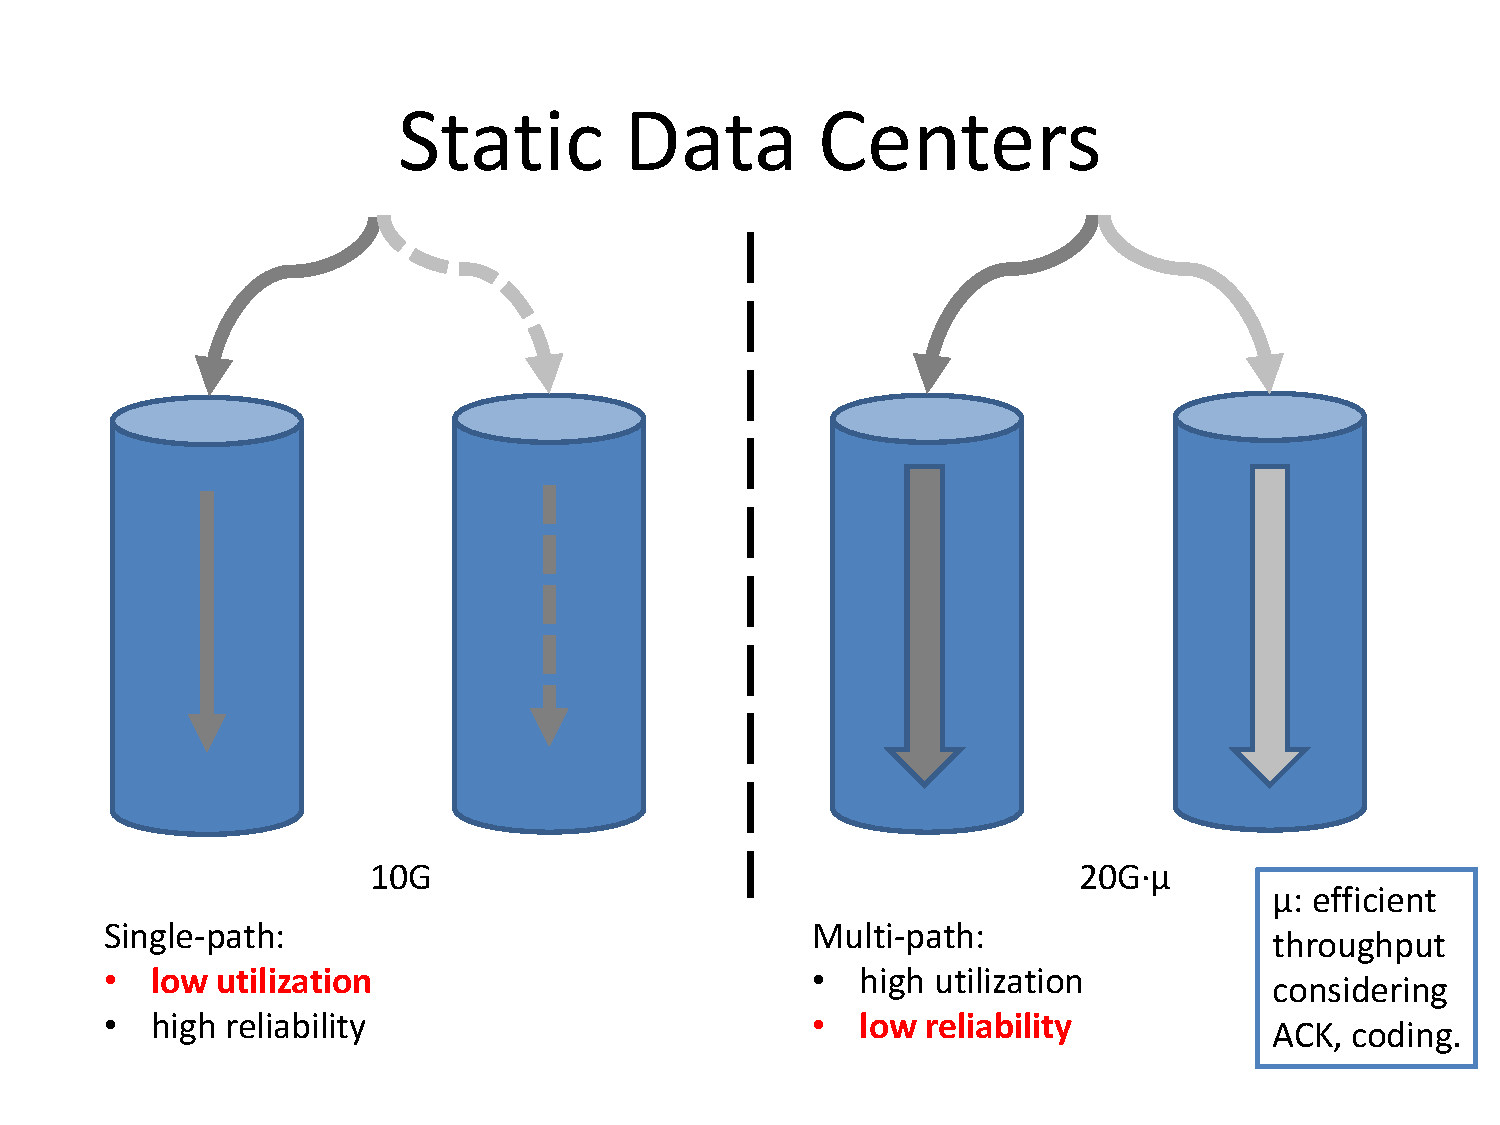
\includegraphics[width=0.8\textwidth]{multipath1.pdf}
\end{figure}
\end{frame}

\begin{frame}{Multi-path TCP in Data Centers}{Low reliability due to drops and retransmission}
\begin{figure}[!t]
\centering
    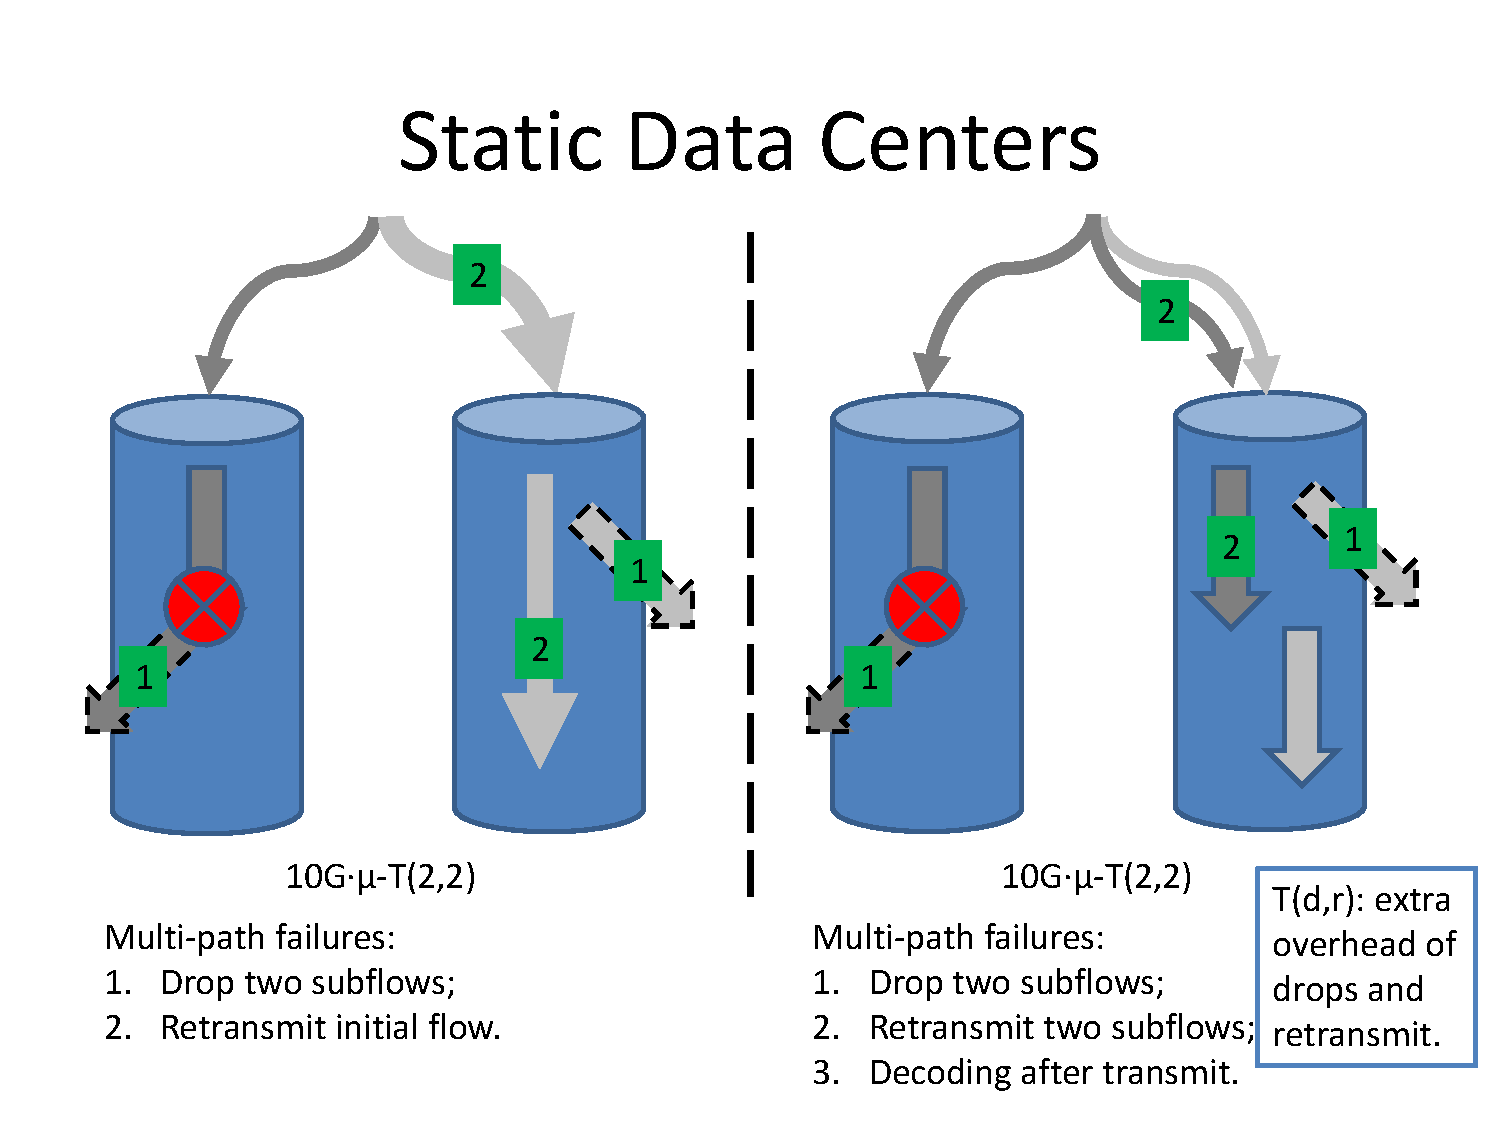
\includegraphics[width=0.8\textwidth]{multipath2.pdf}
\end{figure}
\end{frame}

\begin{frame}{Multi-path TCP in Data Centers}{High reliability through flows backup}
\begin{figure}[!t]
\centering
    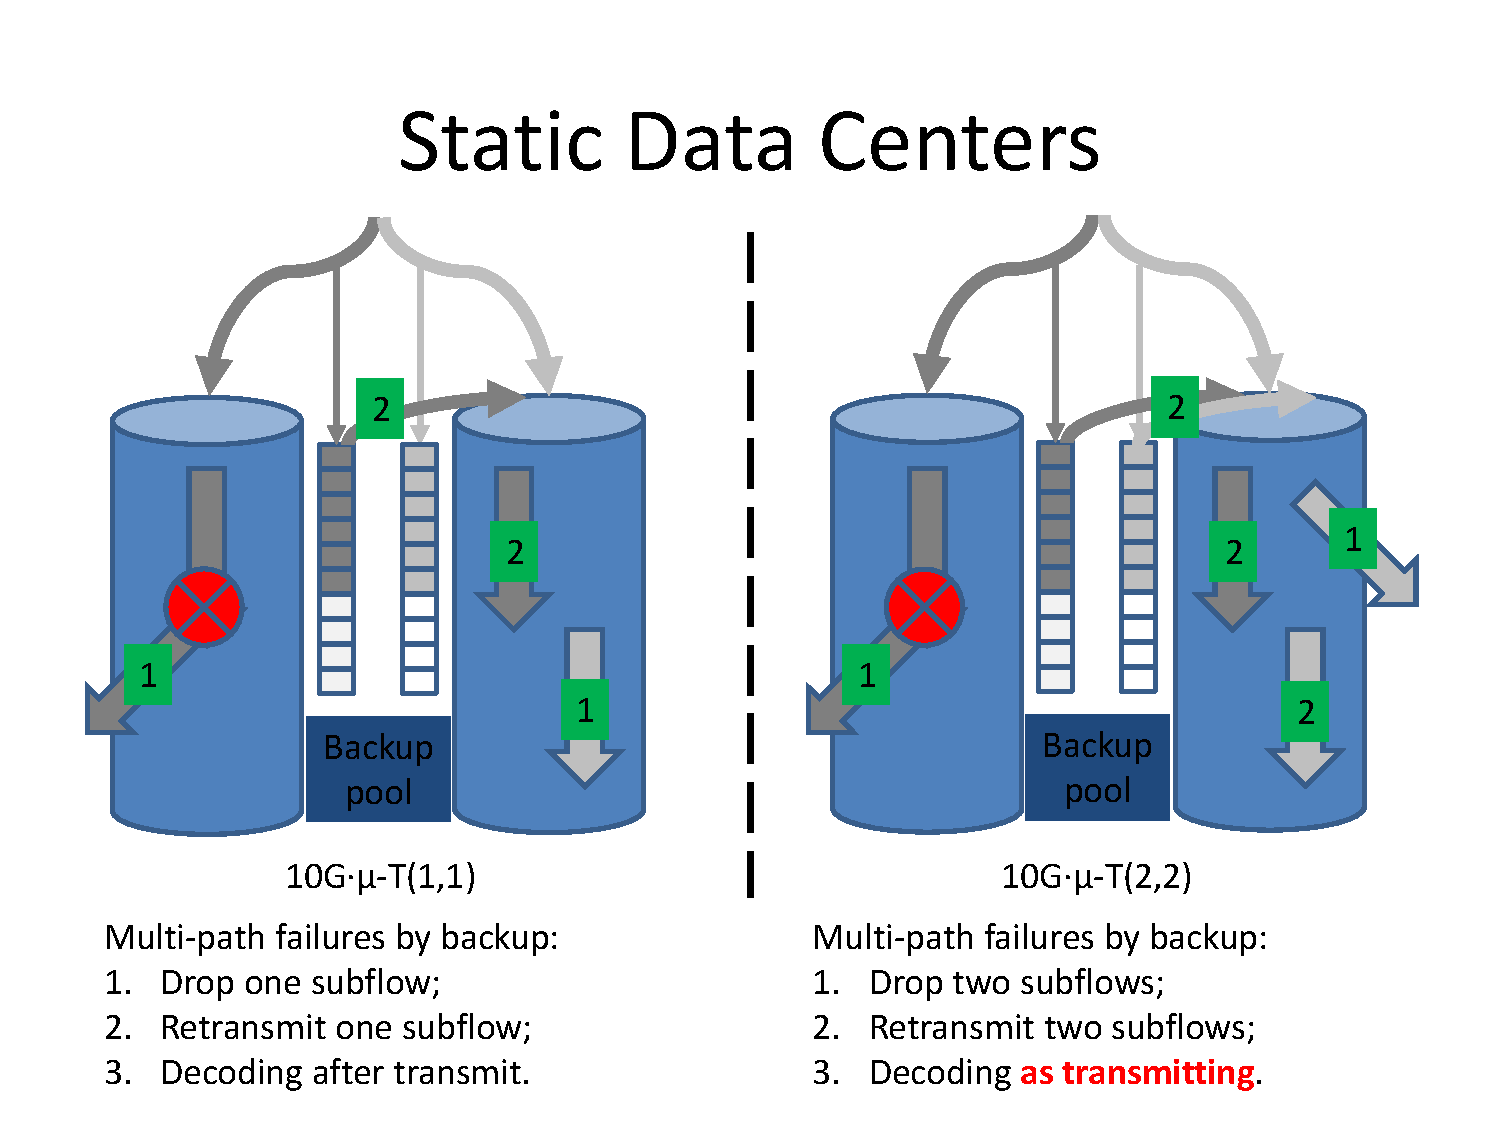
\includegraphics[width=0.8\textwidth]{multipath3.pdf}
\end{figure}
\end{frame}

\begin{frame}{Multi-path TCP in Data Centers}{High efficiency through flexible switching}
\begin{figure}[!t]
\centering
    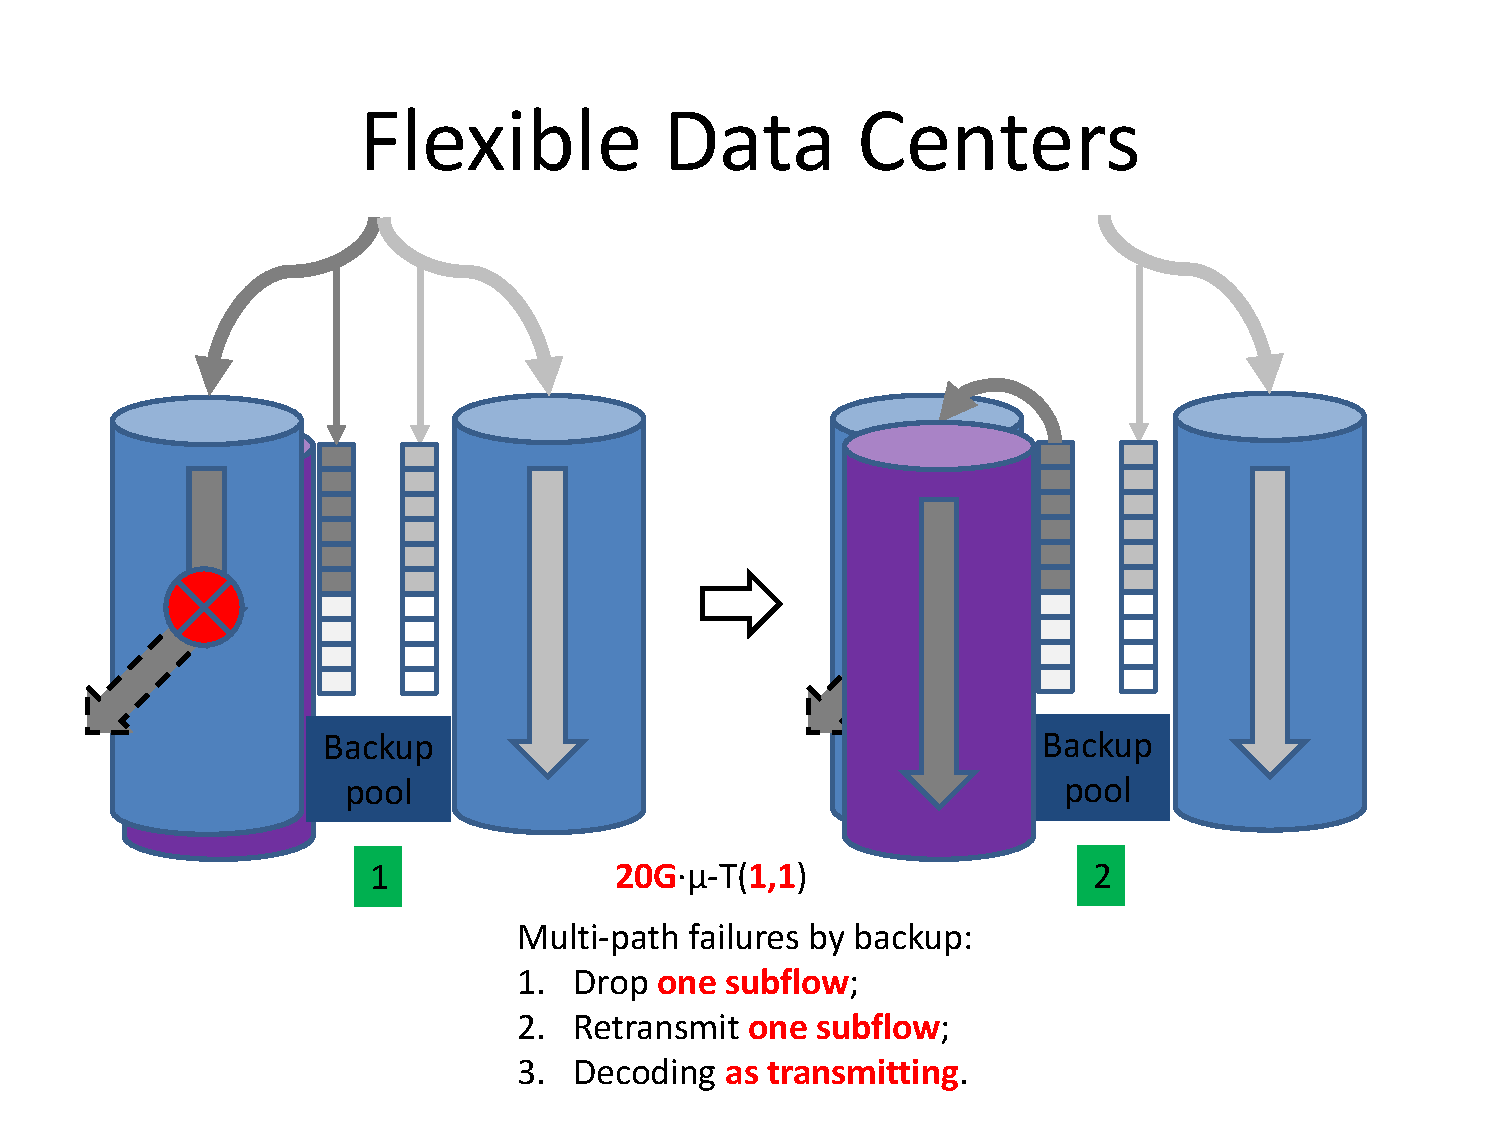
\includegraphics[width=0.8\textwidth]{multipath4.pdf}
\end{figure}
\end{frame}

\begin{frame}{Mtlti-path TCP in Data Centers}
\begin{block}{Failures handling technics}
\begin{itemize}
  \item Flow backup: T(2,2) $\rightarrow$ T(1,1)
  \item Flexible switching: 10G $\rightarrow$ 20G
  \item Block ACK: congestion control
\end{itemize}
\end{block}
\end{frame}
\end{document}


